\section{Aufbau und Durchführung}

Im folgenden Versuch wird eine Kupfer-Röntgenröhre verwendet, dessen Röntgenstrahlen durch ein LiF-Kristall fallen, gebeugt werden und auf ein Geiger-Müller-Zählrohr treffen, welche die Strahlung detektiert.
Die verschiedenen für den Versuch notwendigen Einstellungen können sowohl an der Röntgenröhre, als auch über ein Computerprogramm vorgenommen werden. Zu Beginn wird eine Beschleunigungsspannung $U_{\text{B}} = 35\,\symup{kV}$ 
und ein Emissionsstrom von $I = 1\,\symup{mA}$ für alle weiteren Messungen eingestellt. Weiterhin wird kontrolliert, ob für die Messart $Spektren$ ausgewählt ist und ob sich die $1\,\symup{mm}$ Blende und der Kristall an 
denen für sie vorgesehenen Halterungen des Gerätes befinden.

\begin{figure}[h!]
	\centering
	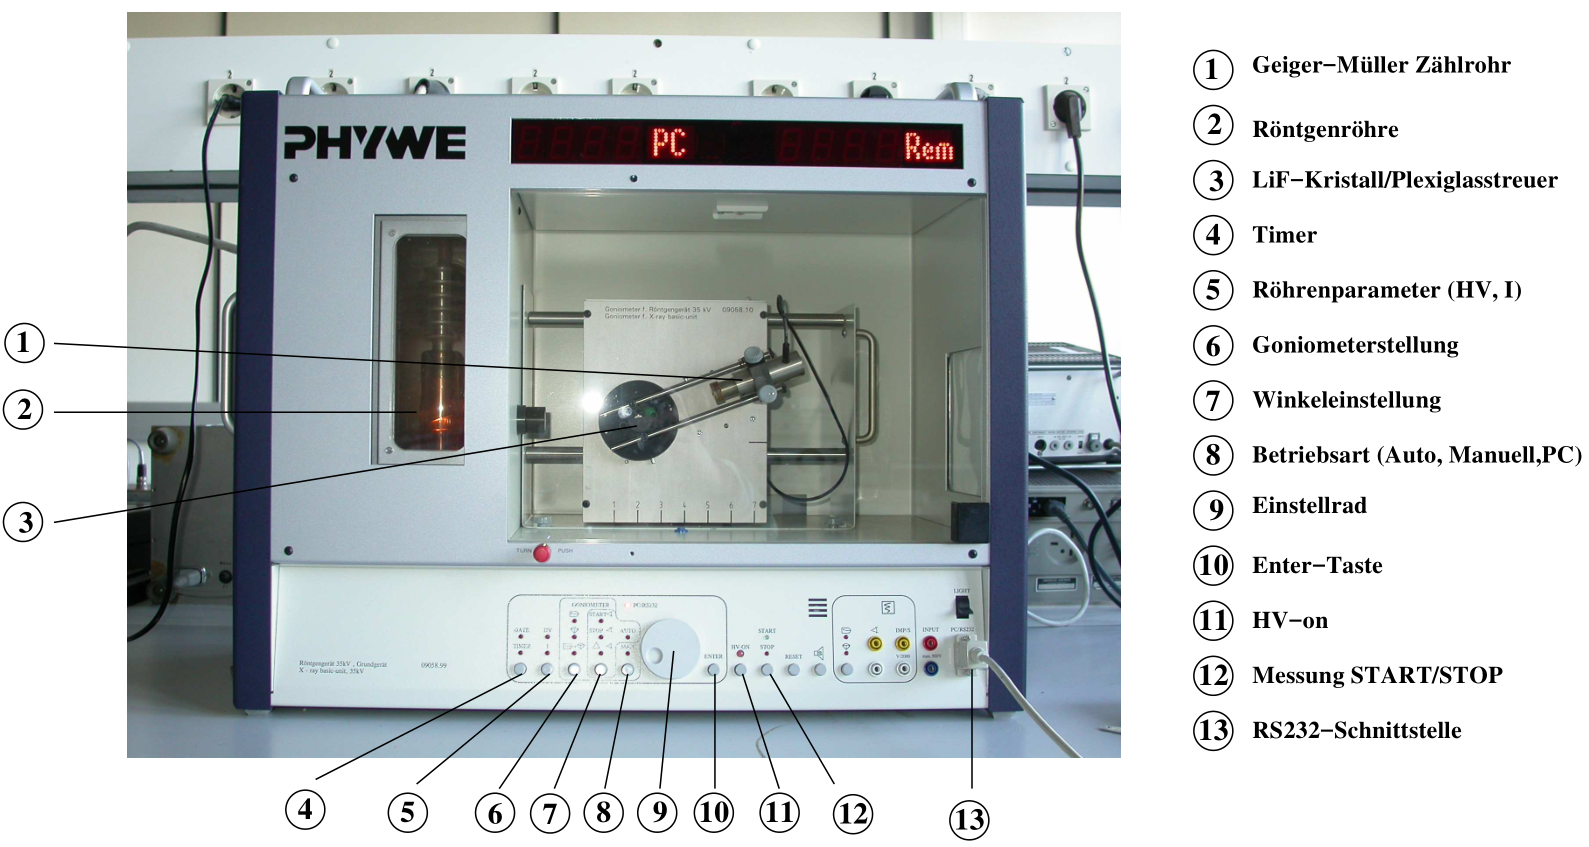
\includegraphics[width=0.9\linewidth]{aufbau.png}
	\caption{Röntgenröhre mit LiF-Kristall und Zählrohr. \cite[4]{anleitung602}}
	\label{fig:aufbau}
\end{figure}

Im ersten Versuchsteil wird zunächst die Braggbedingung überprüft. Dazu wird über das Computerprogramm ein fester Kristallwinkel von $\theta = 14°$ eingestellt. Außerdem wird für das Geiger-Müller-Zählrohr ein Winkelbereich von 
$\alpha_{\text{GM}} = 26°$ bis $\alpha_{\text{GM}} = 30°$ bei einem Winkelzuwachs von $\Delta \alpha_{\text{GM}} = 0{,}1°$ gewählt. Nachdem alle Einstellungen vorgenommen sind, wird die Messung der Strahlungsintensität über 
den Computer gestartet.

Zur Analyse des Röntgenemissionsspektrums wird im Programm der $2\text{:}1 \,\,Koppelmodus$ eingestellt. Der Winkelbereich ist nun $\alpha_{\text{GM}} = 4°$ bis $\alpha_{\text{GM}} = 26°$ mit einem Zuwachs von $\Delta \alpha_{\text{GM}} = 0{,}2°$. Die Integrationszeit
wird auf  $\Delta t = 5\,\symup{s}$ gestellt.

Zuletzt werden verschiedene Absorptionsspektren aufgenommen. Hierfür werden nacheinander unterschiedliche Absorber vor dem Zählrohr angebracht. Es werden die folgenden Materalien und Winkelbereiche verwendet:

\begin{equation}
\begin{aligned}
\text{Brom:}  \,\, \alpha_{\text{Brom}} &= 9°  \,\, \text{bis} \,\, \alpha_{\text{Brom}} = 14° \\
\text{Strontium:} \,\,  \alpha_{\text{Strontium}} &= 9°  \,\, \text{bis} \,\,   \alpha_{\text{Strontium}} = 13° \\
\text{Zirconium:}  \,\, \alpha_{\text{Zirconium}} &= 8°  \,\, \text{bis} \,\,   \alpha_{\text{Zirconium}} = 12° \\
\text{Bismut:} \,\,  \alpha_{\text{Bismut}} &= 11°  \,\, \text{bis} \,\,   \alpha_{\text{Bismut}} = 15° \\
\end{aligned}
\end{equation} 